\section{Body Chapter: Balance of Tasks}
\label{sec:balance}

The study in this section will examine how different amounts of completed interlinear lines affect the integration of machine learning. Budget constraints mean that documentary and descriptive projects rarely have time to interlinearize all the data they record and transcribe. No recommendations about prioritizing tasks are designed for later of integration of machine learning. 

%This main questions that this study asks are: \emph{When faced with limited time, how might integration of machine learning dictate the priorities of segmentation and glossing over free translation? What ratio of these tasks achieves optimal machine learning performance for all tasks?} 
The proposed study will train Transformer models to perform segmentation and glossing and machine translation on Arapaho and Tsez. These two languages have the largest corpora. The models will be trained on different ratios of completed interlinear lines and their results analyzed. The ratio that achieves optimal results on both tasks will indicate how the integration of machine learning should might dictate the priorities of the two tasks.
%contribute to more efficient use of time and budget by providing recommendations

%to determine what balance of effort results in optimal performance. 
Figures \ref{fig:ratio1:1} through \ref{fig:ratio1:15} illustrate how different prioritization of tasks can result in different ratios of completed segmentation/glossing and translation. As an example of how these might come about, let's suppose a documentary team has 40 hours budgeted for interlinearization. The team plans to train a machine learning model to complete missing segmentation, glosses, and free translations. They would like the model to be as accurate as possible. If optimal machine learning performance on each task does not depend on the other lines of interlinearization, then the team should prioritize them equally. Figure \ref{fig:ratio1:1} illustrates the balance of completed interlinear lines when the tasks are prioritized equally. This team needs four times longer to segment and gloss a sentence than to translate it. So they should allot 32 hours for segmentation and glossing and 8 for translation. %This allows them to completely interlinearize 50\% of their transcribed corpus.  
This effort yields the same amount of segmentation/glossing as free translation (a 1:1 ratio).

\begin{figure}[H]
    \centering
    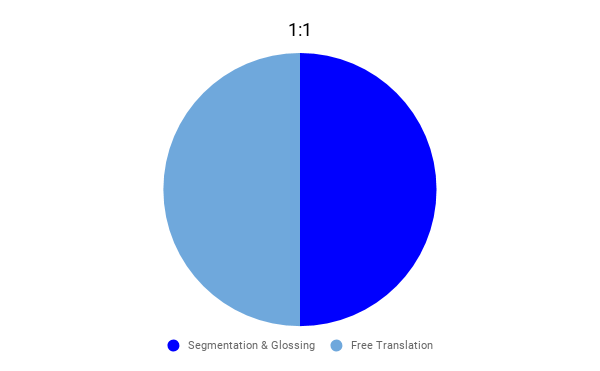
\includegraphics[width=9cm]{figs/Ratio1-1.png}
    \caption[Ratio 1:1 of IGT Completion] {Ratio 1:1 of IGT Completion.}
    \label{fig:ratio1:1}
\end{figure}

If segmented and gloss morphemes are known to help machine learning performance for all interlinear lines, then the team should prioritize segmentation and glossing. Figure \ref{fig:ratio5:1} illustrates a balance of annotation when segmentation/glossing is prioritized. At their rate of work, 38 hours on that task would allow them to segment and gloss about 60\% of the corpus. This would leave 2 hours for translation and allow them to translate about 12\% of the corpus. This effort yields about five times more segmentation/glossing (a 5:1 ratio).

\begin{figure}[H]
    \begin{center}
    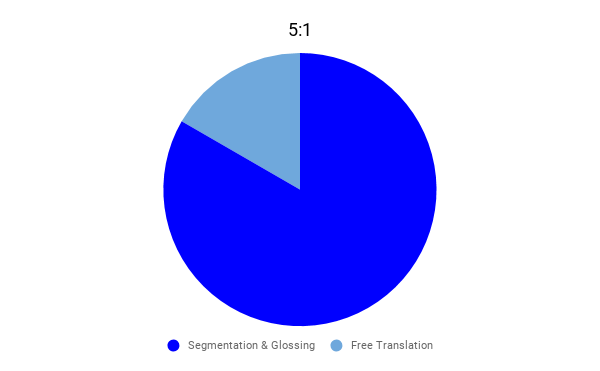
\includegraphics[width=9cm]{figs/Ratio1-5.png}
    \caption[Ratio 5:1 of IGT Completion] {Ratio 5:1 of IGT Completion.}
    \label{fig:ratio5:1}
    \end{center}
\end{figure}

On the other hand, if additional translation was known to improve overall machine learning results, the team should prioritize translation. Figure \ref{fig:ratio2:5} illustrates the outcome of prioritizing translation. The team could translate the whole corpus in 16 hours. With the remaining 24 hours, they could segment and gloss a little less than 40\% of the corpus. This effort would yield nearly three times as many translated lines than segmented/glossed lines (a 2:5 ratio).

\begin{figure}[H]
\begin{center}
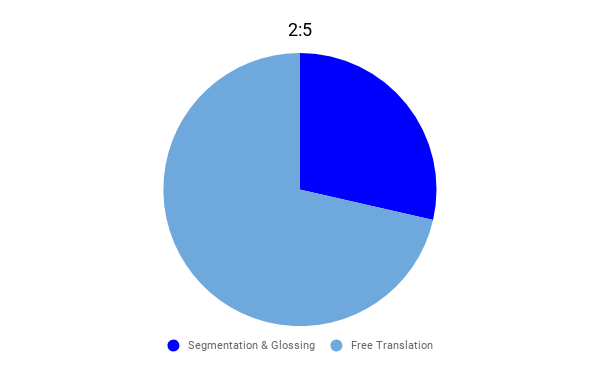
\includegraphics[width=9cm]{figs/Ratio2-5.png}
\caption[Ratio 2:5 of IGT Completion]{Ratio 2:5 of IGT Completion.}
\label{fig:ratio2:5}
\end{center}
\end{figure}

Without prioritizing tasks, projects can easily output very imbalanced IGT. Translation is usually faster and requires less specialized training, so it is easy to spend nearly all the time on translation if the corpus is large. Figure \ref{fig:ratio1:15} illustrates a possible outcome with a large corpus. For example, if our hypothetical team's data doubled in size but its budgeted time did not, it could easily decided to work sequentially and first translate the whole corpus. This would take 32 hours and leave only eight hours for segmentation and glossing.
%becomes almost an afterthought, 
Only about 6\% of the corpus could be segmented and glossed. This yields about 15 times more translated lines than segmented/glossed lines (a 1:15 ratio). 

\begin{figure}[H]
    \begin{center}
    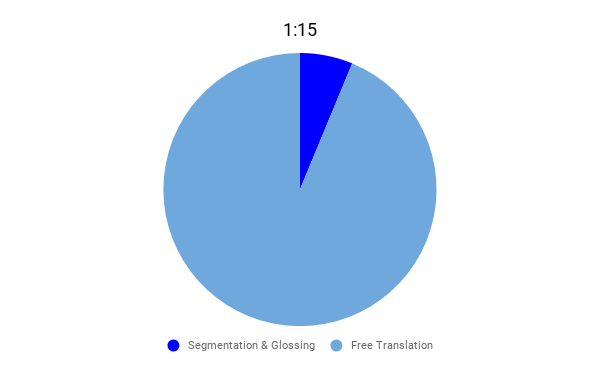
\includegraphics[width=9cm]{figs/Ratio1-15.png}
    \caption[Ratio 1:15 of IGT Completion] {Ratio 1:15 of IGT Completion.}
    \label{fig:ratio1:15}
\end{center}
\end{figure}

Performance of machine learning models in low-resource settings depends on strategic use of limited resources. Four Transformer models will be trained: two for segmentation and glossing and two for machine translation. For each of the two tasks, one model will be trained with information from the other interlinear line(s) and one will be trained without it. Each model will train on as much data that the ratio allows in order to control for differences due to data sizes. The four models are described below. 

\paragraph{Model 1: Segmentation \& Glossing.} 
This experiment assumes that available translations are insufficient to be leveraged for segmentation and glossing. This model will be chosen for each language from the best performing model in section \ref{sec:seggls}. 
%The input will be a character-level representation of the original transcribed text. The output will be labels with morpheme segments and glosses. 
%This model can be run on any proportion of completed IGT. 
If it achieves better performance over Model 2, it will indicate results for automated segmentation and glossing are independent of translation work.

\paragraph{Model 2: Segmentation \& Glossing with Translation.}
Input: transcribed text + translations/POS tags of translation/?
Output: segmented and glossed data
EXAMPLE
This experiment assumes that an equal or higher proportion of translations available. If this consistently achieves better performance than Model 1, it will indicate that LDD projects which wish to integrate machine learning must balance the two tasks as they budget time for interlinearization.

\paragraph{Model 3: Machine Translation.} 
This experiment assumes available glosses are insufficient to leverage for machine translation. This model will take as input the original transcribed text and output an English translation. If this model yields better results than Model 4, it will indicate that results for machine translation are independent of glossed text.

\paragraph{Model 4: Machine Translation with Glosses.}

Translation from the gloss line uses the gloss as input to produce the English translation.This experiment assumes that equal or more glosses are available for each translated line. If this model achieves higher BLEU scores than Model 3, it will indicate a need to balance translation with segmentation and glossing and that machine translation should be added to the LDD workflow after a significant amount of text has been segmented and glossed. 

\begin{singlespace}
\pex<CRFInOut>   
\label{ex:FTgloss}
\a<a> \textbf{INPUT:} \hspace{5 mm} evening \textsc{ins} \textsc{1sg.nom} run \textsc{pfv.pst.sg.fem} in store.\textsc{acc}
\label{ex:FTglossIn}
\a<b> \textbf{OUTPUT:} \hspace{3 mm} In the evening I ran to the store.
\label{ex:FTglossOut}
\xe
\end{singlespace}


\paragraph{Glosses for Machine Translation.}
The secondary questions that this study asks are:
To what extent does leveraging glosses improve machine translation?  To what extent can information extracted from English translations improve segmentation and glossing?

Each model will be tested on the same held-out subset of the data. The segmentation and glossing models will be evaluated by accuracy and Levenshtein distance as described in Section \ref{sec:seggls}. The machine translation models will be evaluated by BLEU \citep{papineni_bleu:_2002} scores.  

The differences in accuracy between different proportions of data and the differences in BLEU scores for the same proportion will be normalized and compared. The results will be extrapolated to determine the ratio that will achieve optimal results on all tasks. 
%Documentary and descriptive linguists will be able take advantage of machine learning. Knowing this optimal ratio will allow them to plan on integrating machine learning into the workflow from the beginning of a field project. 
Although the ratios may change from situation to situation or language to language, this study will provide guidance to linguists as they arrange budgets and timelines.  

\paragraph{Free Translations for Segmentation \& Glossing.}
The proposed research will also look at whether free translations can improve automated segmentation and glossing. This will be done by first running the English free translation through an automated POS tagger and then adding those POS tags as input to the machine translation in addition to the transcribed original text (Model 2). The results will be compared to the Model 1 which only has the original text as input. Evaluation will be done with F$_1$-scores, accuracy, and Levenshtein distance between Models 1 and 2 on the same test sets in a 10-fold cross validation. 

This research will also look at how glosses can be leveraged to improve machine translations and how information from the free translation, such as English POS tags, can improve automated morpheme segmentation and glossing. This will be done by comparing two machine translation models using as input 1) just the original text (Model 3) and 2) just the glosses (Model 4). Evaluation will be based on BLEU scores on same test sets in a 10-fold cross validation. 

Leveraging glosses to improve low-resource machine translation has been used successfully in statistical machine translation XXX. The strategy leverages glossed morpheme segments, essentially treating the gloss line as noisy, ungrammatical English to be denoised (Xie et al. 2018). This is illustrated in (2), using the labeled analysis in (1). The motivation to use the gloss line in the translation task is that the glosses produced have already transformed the source language into a form that is closer to the target language. They also communicate morphological information about the source words. Other approaches used when dealing with morphologically complex languages have used compound splitting (Koehn and Knight, 2003; Macherey et al., 2011) and stemming (Fraser and Marcu 2005) to reduce vocabulary size of the more morphologically complex language, and Byte-Pair (BPE) encoding of subwords in the source language (Sennrich et al., 2015). 

\subsection{Pilot Study: Balance of Tasks}

ENTER TEXT